\documentclass[10pt,letterpaper]{article}
\usepackage[T1]{fontenc}
\usepackage[utf8]{inputenc}
\usepackage{lmodern}
\usepackage[margin=0.82in,headheight=15pt]{geometry}
\usepackage{microtype}
\usepackage{amsmath,amssymb,amsthm,mathtools}
\usepackage{booktabs,longtable,array,tabularx}
\usepackage{enumitem}
\usepackage{xcolor}
\usepackage{tikz}
\usetikzlibrary{calc,intersections,arrows.meta,positioning}
\usepackage{listings}
\usepackage{fancyhdr}
\usepackage{hyperref}
\usepackage[nameinlink,capitalize,noabbrev]{cleveref}
\usepackage{bookmark}
\usepackage{url}

\definecolor{linkblue}{RGB}{25,75,140}
\definecolor{codegray}{RGB}{245,245,245}
\hypersetup{colorlinks=true,linkcolor=linkblue,citecolor=linkblue,urlcolor=linkblue,pdfauthor={OpenAI},pdftitle={Eight classical geometry theorems in intuitionistic primitive recursive arithmetic}}
\pagestyle{fancy}
\fancyhf{}
\lhead{Constructive projective and affine geometry in iPRA}
\rhead{\thepage}
\setlength{\parindent}{0pt}
\setlength{\parskip}{0.55em}
\setlist{nosep,leftmargin=1.6em}
\lstset{basicstyle=\ttfamily\small,backgroundcolor=\color{codegray},frame=single,breaklines=true,columns=fullflexible,keepspaces=true}

\newtheorem{theorem}{Theorem}[section]
\newtheorem{lemma}[theorem]{Lemma}
\newtheorem{proposition}[theorem]{Proposition}
\newtheorem{corollary}[theorem]{Corollary}
\theoremstyle{definition}
\newtheorem{definition}[theorem]{Definition}
\newtheorem{remark}[theorem]{Remark}
\newtheorem{construction}[theorem]{Construction}

\newcommand{\F}{\mathbb F}
\newcommand{\Q}{\mathbb Q}
\newcommand{\Z}{\mathbb Z}
\newcommand{\N}{\mathbb N}
\newcommand{\ipra}{\mathrm{iPRA}}
\newcommand{\br}[3]{[\,#1\,#2\,#3\,]}
\newcommand{\crat}[4]{(#1,#2;#3,#4)}
\newcommand{\join}{\mathbin{\vee}}
\newcommand{\meet}{\mathbin{\wedge}}
\newcommand{\cross}{\mathbin{\times}}
\newcommand{\Rat}{\operatorname{Rat}}
\newcommand{\Inc}{\operatorname{Inc}}
\newcommand{\Col}{\operatorname{Col}}
\newcommand{\Con}{\operatorname{Con}}
\newcommand{\Area}{\operatorname{Area}}
\newcommand{\poly}{\operatorname{Poly}}
\newcommand{\code}[1]{\texttt{#1}}
\newcommand{\todoFormal}{\textsf{formalization obligation}}

\title{Eight Classical Geometry Theorems in Intuitionistic Primitive Recursive Arithmetic\\
\large Pappus harmonic, Ceva, Menelaus, Carnot conic and polygon, Hoehn, Pappus hexagon, and Brianchon}
\author{Constructive proof development and Lean formalization plan}
\date{15 November 2026}

\begin{document}
\maketitle

\begin{abstract}
We give constructive, division-controlled proofs of eight classical incidence and ratio theorems in a form that is directly arithmetizable in intuitionistic primitive recursive arithmetic.  The internal universe is the rational affine or projective plane, more generally any fixed primitively presented field of characteristic zero.  Every geometric object is a finite tuple of number codes; every incidence assertion is a polynomial equality; every nondegeneracy assumption is an explicit apartness hypothesis; and every existential conclusion is accompanied by a primitive-recursive witness.  The only unbounded family, Carnot's polygon theorem, is formulated with explicit side-factorization certificates and proved by quantifier-free induction on finite products.  No appeal is made to excluded middle for arbitrary propositions, choice, completeness of the reals, or the fundamental theorem of algebra.

The coordinate kernels are independently checked by the accompanying SymPy script.  A Lean 4 outline isolates the generic field-level geometry from the final arithmetization through the current \texttt{ConciseIPRA} bi-interpretation.  The document is intentionally honest about status: it contains complete human proofs and executable algebra certificates, while the final native \texttt{ConciseIPRA} derivation files remain a clear, finite implementation task rather than a completed formalization.
\end{abstract}

\tableofcontents
\newpage

\section{Scope, exact meaning, and theorem inventory}

\subsection{What ``proved in \texorpdfstring{$\ipra$}{iPRA}'' means here}

A literal theorem of first-order arithmetic cannot quantify over an unstructured continuum of Euclidean points.  We therefore use the standard arithmetized reading:

\begin{quote}
A point, line, conic, polynomial, or finite polygon is represented by a natural-number code.  The field operations, tuple projections, determinants, cross products, polynomial composition, and finite products are primitive-recursive functions of those codes.  The geometric theorem is the corresponding arithmetical implication between code predicates.
\end{quote}

The canonical field is $\Q$.  The same proof is uniform for any fixed field whose carrier and operations are primitively presented and whose field laws have been verified in $\ipra$.  This includes fixed number fields, so the restriction to rational coordinates is not a restriction to ruler-only configurations; it is the cleanest literal internal model.  Externally, every proof below is a field identity and hence remains valid over any characteristic-zero field and over constructive real-number structures whenever the named denominators are apart from zero.

The projective theorems are stated with homogeneous coordinates.  The affine ratio theorems are first stated with \emph{directed} ratios.  For an ordered convex configuration, the directed factors have the signs shown in the diagram, and the displayed MathWorld formulas with ordinary positive lengths follow immediately.  This separation is important constructively: order and absolute value are not needed for the algebraic core.

\subsection{Status table}

\begin{longtable}{p{0.19\textwidth}p{0.23\textwidth}p{0.25\textwidth}p{0.23\textwidth}}
\toprule
Theorem & Constructive internal form & Main certificate & Existential witness \\
\midrule
\endhead
Pappus harmonic & Four collinear projective points have cross-ratio $-1$ & A three-cross-product coordinate calculation & The harmonic point $W\sim(t,0,2t-1)$ \\
Ceva & Three rational cevians are concurrent iff a cross-multiplied product identity holds & Determinant of three line covectors & Explicit common point $P$ \\
Menelaus & Three side points are collinear iff the directed product is $-1$ & Determinant of their three point vectors & Explicit line $D\join E$ \\
Carnot conic & Six side points lie on a conic iff the product condition holds & Three binary-quadratic factorizations & Six explicit conic coefficients \\
Carnot polygon & A certified degree-$n$ restriction on every side gives the circular product $(-1)^{mn}$ & Endpoint evaluation of a supplied factorization & The intersection parameters are input data \\
Hoehn & Two pentagram products of five signed ratios are $1$ & Cyclic determinant cancellation & Each $W_i$ is a cross product of two joins \\
Pappus hexagon & Three opposite-side intersections are collinear & The vector identity $X-Y+Z=0$ & All three intersections are explicit cross products \\
Brianchon & Three opposite-vertex diagonals of a circumscribed hexagon are concurrent & Pascal's polynomial identity in the dual plane & The concurrency point is the meet of two diagonals \\
\bottomrule
\end{longtable}

\subsection{Constructive strength actually used}

The fixed-size theorems use only:
\begin{enumerate}
\item equations in a commutative field;
\item cancellation under an explicit nonzero hypothesis;
\item finite tuple manipulation; and
\item explicit construction of intersections, joins, and coefficients.
\end{enumerate}
Carnot's polygon theorem additionally uses primitive recursion on the two finite indices and quantifier-free induction for the telescoping product.  Thus the arguments fit not merely classical PRA but intuitionistic PRA.  No step invokes $P\lor\neg P$ for an arbitrary formula.  Equality and order of rational codes are decidable, but that is a primitive-recursive fact about the chosen data type, not an appeal to global excluded middle.

\subsection{Nondegeneracy discipline}

Every quotient in an informal geometry book hides a nonzero premise.  We expose those premises.  Typical examples are:
\begin{itemize}
\item a projective point or line vector is nonzero;
\item two points used to define a line are distinct;
\item two lines used to define an intersection are distinct;
\item a side point is not a triangle vertex, so both of its nonzero barycentric coordinates are apart from zero;
\item a curve avoids every polygon vertex, so no side parameter is $0$ or $1$; and
\item in the affine Hoehn theorem, the relevant diagonal intersections are finite.
\end{itemize}
The division-free equalities remain meaningful in some degenerate cases, but the named geometric ratios do not.  The report proves the strongest clean theorem with all ratios defined, and records where the polynomial identity itself survives beyond that domain.

\section{Primitive-recursive coordinate framework}

\subsection{Integer and rational codes}

One convenient implementation avoids quotient types.  An integer is a signed natural pair, or equivalently the usual even--odd code.  A rational is a pair $(a,b)$ with $a\in\Z$ and $b\in\N_{>0}$, read as $a/b$.  Equality is
\[
(a,b)\equiv(c,d)\quad:\Longleftrightarrow\quad ad=cb.
\]
Addition and multiplication are
\[
(a,b)+(c,d)=(ad+cb,bd),\qquad (a,b)(c,d)=(ac,bd).
\]
For $a\ne0$, the inverse is obtained by swapping numerator and denominator and moving the sign to the numerator.  Normalization by a gcd is optional; none of the proofs requires canonical representatives.  All operations, predicates, and denominator-positivity checks are primitive recursive.  Field equality is a polynomial equality over signed integers.

Fixed-length tuples are encoded by any standard primitive-recursive pairing function.  Consequently vectors in $\Q^2$ or $\Q^3$, $3\times3$ matrices, and finite coefficient lists are all natural-number objects inside $\ipra$.

\subsection{Projective points and lines}

A projective point is a nonzero vector $P=(p_0,p_1,p_2)\in\F^3$, modulo nonzero scalar multiplication.  A projective line is a nonzero covector $\ell=(\ell_0,\ell_1,\ell_2)$, also modulo scale.  Incidence is the equation
\[
\Inc(P,\ell):\quad \ell\cdot P=0.
\]
Because points and lines are both represented by triples, duality is literal syntax.  Define
\[
P\join Q:=P\cross Q,\qquad \ell\meet m:=\ell\cross m,
\]
where
\[
(u_0,u_1,u_2)\cross(v_0,v_1,v_2)
=(u_1v_2-u_2v_1,\;u_2v_0-u_0v_2,\;u_0v_1-u_1v_0).
\]
The cross product is a fixed polynomial map.  The determinant bracket is
\[
\br{P}{Q}{R}:=\det(P,Q,R)=P\cdot(Q\cross R).
\]
Then
\[
\Col(P,Q,R)\Longleftrightarrow\br{P}{Q}{R}=0,
\qquad
\Con(\ell,m,n)\Longleftrightarrow\det(\ell,m,n)=0.
\]
Whenever the two inputs are distinct, $P\join Q$ is a nonzero line and $\ell\meet m$ is a nonzero point.  The proof that each input is incident with its join or meet is a direct ring identity.

\subsection{Affine points, signed area, and directed ratios}

An affine point $(x,y)$ is embedded as $\widetilde P=(x,y,1)$.  For affine points $A,B,C$, write
\[
[ABC]:=\det(\widetilde A,\widetilde B,\widetilde C)
       =\det(B-A,C-A).
\]
This is twice the oriented Euclidean area, but only its algebraic properties matter.

For distinct affine points $U,V$, a point $X$ on their line has a parameter $t$ when
\[
X=(1-t)U+tV.
\]
The directed ratio is
\[
\frac{UX}{XV}:=\frac{t}{1-t}.
\]
A quotient-free version stores a numerator--denominator pair $(t,1-t)$.  In all theorem statements, the nonzero premises $t\ne0$ and $1-t\ne0$ are explicit when the ratio is used.

If $X$ is given projectively as
\[
\widetilde X\sim \alpha\widetilde U+\beta\widetilde V,
\qquad \alpha+\beta\ne0,
\]
then $t=\beta/(\alpha+\beta)$ and $UX/XV=\beta/\alpha$.  This observation converts cross-product intersection formulas directly into segment ratios.

\subsection{Conics and polynomial curves}

A projective conic is represented by the homogeneous quadratic
\[
Q(x,y,z)=ux^2+vy^2+wz^2+p yz+q zx+r xy.
\]
We do not divide the mixed coefficients by $2$; this keeps every formula integral and also avoids an irrelevant characteristic-$2$ convention.  A conic may be degenerate.  It avoids the coordinate vertices exactly when $u,v,w$ are nonzero.

A plane polynomial curve is represented by a finite coefficient list.  If $F(x,y)$ has total degree at most $n$ and $U,V$ are affine points, the side restriction
\[
g(T)=F((1-T)U+TV)
\]
is computed by a primitive-recursive coefficient transformation.  Equality of two restrictions means equality of their coefficient lists, not an extensional quantification over all field elements.

\subsection{Projective and affine normalization are constructive}

The coordinate normalizations used below are explicit inverses of small matrices.

For an affine frame $A,B,Z$ with $[ABZ]\ne0$, the map
\[
P\longmapsto \begin{pmatrix}B-A&Z-A\end{pmatrix}^{-1}(P-A)
\]
sends $A$ to $(0,0)$, $B$ to $(1,0)$, and $Z$ to $(0,1)$.  The inverse is the adjugate divided by the nonzero determinant.

For two distinct projective lines, choose their intersection $O$ and one named point away from $O$ on each line.  These three noncollinear vectors form a basis.  In that basis the two lines are coordinate lines, and any other named point on either line has the form used in the Pappus calculation.  Again the transformation is an explicit matrix inverse.

Thus normalization introduces no choice principle.  It is a primitive-recursive term under the displayed determinant-apartness assumptions.

\section{Algebraic lemmas used repeatedly}

\begin{lemma}[Join--meet identities]
For all $U,V,W\in\F^3$,
\[
U\cdot(U\cross V)=V\cdot(U\cross V)=0,
\qquad
\br{U}{V}{W}=U\cdot(V\cross W).
\]
If $U\cross V\ne0$, it represents the unique projective line through $U$ and $V$; dually for the meet of two lines.
\end{lemma}

\begin{proof}
The two dot products expand to the same two monomials with opposite signs.  The determinant identity is the definition of the $3\times3$ determinant.  For uniqueness, a line through $U,V$ is a nonzero solution of two homogeneous linear equations.  When $U,V$ are independent, their common orthogonal space is one-dimensional, and the explicit nonzero solution is $U\cross V$.  Over $\Q$ this finite-dimensional claim is proved constructively by choosing a nonzero $2\times2$ minor, a decidable finite case split.
\end{proof}

\begin{lemma}[Intersection parameter]
Let $A,B,C,D$ be affine points, with $A\ne B$, and let $X=AB\cap CD$ be finite.  Put
\[
L(P):=[CDP].
\]
If $X=(1-t)A+tB$, then
\[
(1-t)L(A)+tL(B)=0,
\qquad
\frac{AX}{XB}=-\frac{L(A)}{L(B)}.
\]
The division-free form is $tL(B)=-(1-t)L(A)$.
\end{lemma}

\begin{proof}
The bracket is affine-linear in its third point because all affine representatives have final coordinate $1$.  Since $X$ lies on $CD$, $L(X)=0$.  Substitution gives the first equation.  The second is merely the definition $AX/XB=t/(1-t)$, cross-multiplied before any cancellation.
\end{proof}

\begin{lemma}[Area principle]
Suppose $P=A_1A_2\cap BC$ and all named ratios are defined.  Then
\[
\frac{A_1P}{PA_2}=\frac{[A_1BC]}{[A_2CB]}.
\]
Equivalently, after choosing a consistent line orientation, the directed ratio of the two collinear segments equals the ratio of the two signed areas on the common base $BC$.
\end{lemma}

\begin{proof}
Apply the preceding lemma to the line functional $L(X)=[BCX]$.  The apparent sign difference between common textbook formulas is only the choice between $PA_2$ and $A_2P$.
\end{proof}

\begin{lemma}[Binary quadratic root product, division-free]
Let
\[
h(y,z)=v y^2+p yz+wz^2.
\]
Suppose $h(y_1,z_1)=h(y_2,z_2)=0$ and the two projective points are distinct, so
$\delta=y_1z_2-y_2z_1\ne0$.  Then
\[
v y_1y_2=wz_1z_2.
\]
\end{lemma}

\begin{proof}
Multiply the first root equation by $y_2z_2$, the second by $y_1z_1$, and subtract.  The result factors as
\[
y_2z_2h(y_1,z_1)-y_1z_1h(y_2,z_2)
=(y_1z_2-y_2z_1)(v y_1y_2-wz_1z_2).
\]
The left side is zero.  Cancel the explicitly nonzero factor $\delta$.
\end{proof}

\begin{lemma}[Certified side product]
Let a univariate polynomial restriction be supplied with the coefficient identity
\[
g(T)=c\prod_{j=1}^{n}(T-t_j),\qquad c\ne0,
\]
and suppose $g(0),g(1)\ne0$.  Then
\[
\prod_{j=1}^{n}\frac{t_j}{1-t_j}
=(-1)^n\frac{g(0)}{g(1)}.
\]
\end{lemma}

\begin{proof}
Coefficient equality permits evaluation at $0$ and $1$:
\[
g(0)=c(-1)^n\prod_jt_j,
\qquad
g(1)=c\prod_j(1-t_j).
\]
The endpoint assumptions imply each denominator is nonzero.  Cancel $c$ and cross-multiply.  The same proof is a primitive recursion on the list $t_1,\ldots,t_n$.
\end{proof}

\begin{lemma}[Duality is syntactic]
Any theorem expressed solely with cross products, determinants, incidence, collinearity, and concurrency has a dual obtained by exchanging point vectors with line vectors and exchanging join with meet.  A determinant proof of the original theorem is literally a determinant proof of the dual.
\end{lemma}

\begin{proof}
Both points and lines are nonzero triples, and both join and meet are the same polynomial operation $\cross$.  Collinearity and concurrency are both vanishing of a $3\times3$ determinant.  No semantic completeness theorem for projective geometry is required.
\end{proof}

\section{Pappus's harmonic theorem}

\subsection{Constructive statement}

Let $A,B,Y$ be distinct collinear affine points, let $Z$ be off their line, and let $D$ be a point of $AZ$ distinct from $A,Z$.  Define
\[
C=DY\cap ZB,
\qquad X=AC\cap DB,
\qquad W=ZX\cap AB,
\]
with the displayed intersections nondegenerate.  Then the four points $A,B,W,Y$ form a harmonic range:
\[
\crat{A}{B}{W}{Y}=-1.
\]
In the MathWorld order $A-W-B-Y$, this says that the three directed lengths $AW,AB,AY$ are in harmonic progression.

\begin{center}
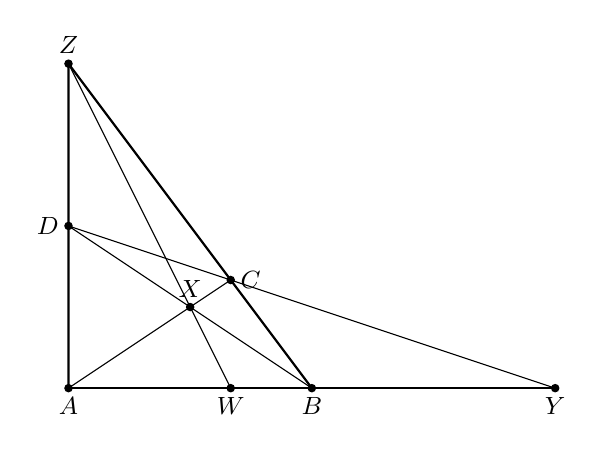
\begin{tikzpicture}[scale=1.03, every node/.style={font=\small}]
  \coordinate (A) at (0,0);
  \coordinate (W) at (2,0);
  \coordinate (B) at (3,0);
  \coordinate (Y) at (6,0);
  \coordinate (Z) at (0,4);
  \coordinate (D) at (0,2);
  \coordinate (C) at (2,1.3333);
  \coordinate (X) at (1.5,1);
  \draw[thick] (A)--(Y);
  \draw[thick] (A)--(Z)--(B);
  \draw (D)--(Y);
  \draw (A)--(C);
  \draw (D)--(B);
  \draw (Z)--(W);
  \foreach \P/\pos in {A/below,W/below,B/below,Y/below,Z/above,D/left,C/right,X/above}
    {\fill (\P) circle (1.5pt) node[\pos] {$\P$};}
\end{tikzpicture}
\end{center}

\subsection{Coordinate proof}

Apply the constructive affine normalization of the previous section:
\[
A=(0,0,1),\quad B=(1,0,1),\quad Z=(0,1,1).
\]
Because $Y\in AB$ and $D\in AZ$, write
\[
Y=(t,0,1),\qquad D=(0,d,1),
\]
where $d\ne0,1$.  Repeated use of join and meet gives representatives
\begin{align*}
C&=(D\join Y)\meet(Z\join B)\\
 &\sim\bigl(t(d-1),\;-d(t-1),\;d-t\bigr),\\[0.3em]
X&=(A\join C)\meet(D\join B)\\
 &\sim\bigl(-dt(d-1),\;d^2(t-1),\;-d(dt-2t+1)\bigr),\\[0.3em]
W&=(Z\join X)\meet(A\join B)\\
 &\sim -d(d-1)\bigl(t,0,2t-1\bigr).
\end{align*}
Since $d(d-1)\ne0$, we may take
\[
W\sim(t,0,2t-1).
\]
In particular, $W$ is independent of the auxiliary choice of $D$.

Identify the projective baseline $AB$ with $\mathbf P^1$ by retaining the first and third homogeneous coordinates.  Thus
\[
A=(0:1),\quad B=(1:1),\quad Y=(t:1),\quad W=(t:2t-1).
\]
For two line points $P=(p_0:p_1)$ and $Q=(q_0:q_1)$ write
$[P,Q]=p_0q_1-p_1q_0$.  The division-free harmonic condition is
\[
[A,W][B,Y]+[A,Y][B,W]=0.
\]
Here
\[
[A,W]=-t,\quad [B,Y]=1-t,\quad [A,Y]=-t,\quad [B,W]=t-1,
\]
and the sum is zero.  Therefore $\crat{A}{B}{W}{Y}=-1$.

If $2t-1\ne0$, then $W$ is finite with affine coordinate
\[
w=\frac{t}{2t-1}.
\]
Taking $AB=1$ and $AY=t$ gives
\[
\frac1{AW}+\frac1{AY}=\frac{2t-1}{t}+\frac1t=2=\frac2{AB},
\]
which is exactly the harmonic-progression formulation appearing in elementary accounts.

\subsection{Constructive audit}

The proof consists of fixed polynomial expressions and one cancellation by $d(d-1)\ne0$.  The harmonic conclusion is stated without division and therefore also covers the case $2t-1=0$, where $W$ is the point at infinity of $AB$.  No order or betweenness argument is used; the picture's order is only needed to reinterpret the directed relation as a positive-length harmonic progression.

\section{Ceva's theorem and Menelaus' theorem}

Both theorems become one-line determinant criteria in barycentric coordinates.  This is preferable to proofs by areas because the converses and all signs are automatic.

\subsection{Barycentric setup}

Normalize the reference triangle projectively as
\[
A=(1,0,0),\qquad B=(0,1,0),\qquad C=(0,0,1).
\]
Let
\[
D=(0,d_B,d_C)\in BC,\quad
E=(e_A,0,e_C)\in CA,\quad
F=(f_A,f_B,0)\in AB,
\]
where every displayed coordinate is nonzero.  Then the directed side ratios are
\[
\frac{BD}{DC}=\frac{d_C}{d_B},\qquad
\frac{CE}{EA}=\frac{e_A}{e_C},\qquad
\frac{AF}{FB}=\frac{f_B}{f_A}.
\]
These equalities are definitions of barycentric side coordinates and can be kept cross-multiplied.

\subsection{Ceva}

\begin{theorem}[Constructive Ceva]
The cevians $AD,BE,CF$ are concurrent if and only if
\[
d_Ce_Af_B=d_Be_Cf_A.
\]
Equivalently,
\[
\frac{BD}{DC}\frac{CE}{EA}\frac{AF}{FB}=1.
\]
\end{theorem}

\begin{proof}
The three cevian lines have covectors
\[
AD=(0,-d_C,d_B),\qquad
BE=(e_C,0,-e_A),\qquad
CF=(-f_B,f_A,0).
\]
Their determinant is
\[
\det\begin{pmatrix}
0&-d_C&d_B\\
e_C&0&-e_A\\
-f_B&f_A&0
\end{pmatrix}
=d_Be_Cf_A-d_Ce_Af_B.
\]
Thus concurrency implies the displayed product identity.

For the converse, assume the identity and define the explicit point
\[
P=(e_Ad_C,\;d_Be_C,\;d_Ce_C).
\]
It is nonzero.  Direct substitution gives
\begin{align*}
AD\cdot P&=-d_Cd_Be_C+d_Bd_Ce_C=0,\\
BE\cdot P&=e_Ce_Ad_C-e_Ad_Ce_C=0,\\
CF\cdot P&=-f_Be_Ad_C+f_Ad_Be_C=0,
\end{align*}
where the final equality is exactly the hypothesis.  Hence all three cevians pass through $P$.
\end{proof}

This proof supplies the concurrency witness rather than deriving its existence indirectly.  It is therefore intuitionistically stronger than a bare determinant-zero argument.

\subsection{Menelaus}

\begin{theorem}[Constructive Menelaus]
The points $D,E,F$ are collinear if and only if
\[
d_Be_Cf_A+d_Ce_Af_B=0.
\]
Equivalently, in directed ratios,
\[
\frac{BD}{DC}\frac{CE}{EA}\frac{AF}{FB}=-1.
\]
When exactly one of $D,E,F$ lies on an extended side outside the triangle, taking ordinary positive lengths removes the minus sign and gives the customary MathWorld equality of the two triple products.
\end{theorem}

\begin{proof}
The determinant of the three point vectors is
\[
\det\begin{pmatrix}
0&e_A&f_A\\
d_B&0&f_B\\
d_C&e_C&0
\end{pmatrix}
=d_Be_Cf_A+d_Ce_Af_B.
\]
Hence collinearity is equivalent to the stated polynomial equation.

For a completely explicit converse, the line through $D$ and $E$ is
\[
D\join E=(d_Be_C,\;d_Ce_A,\;-d_Be_A).
\]
Its value at $F$ is
\[
(d_Be_C)f_A+(d_Ce_A)f_B,
\]
which vanishes precisely under the Menelaus identity.  Thus $F$ lies on $DE$.
\end{proof}

\subsection{Relation between the two signs}

Ceva and Menelaus differ only in whether the relevant $3\times3$ matrix contains line covectors or point vectors.  In the first determinant the two contributing monomials have opposite signs; in the second they have the same sign.  This is the coordinate source of the familiar $+1$ versus $-1$ distinction in directed-ratio formulations.

\section{Carnot's conic theorem}

\subsection{Constructive statement}

Use the same barycentric triangle $A=(1,0,0)$, $B=(0,1,0)$, $C=(0,0,1)$.  Let
\begin{align*}
D_i&=(0,d_i,e_i)\in BC,\\
E_i&=(a_i,0,c_i)\in CA,\\
F_i&=(p_i,q_i,0)\in AB,
\end{align*}
for $i=1,2$.  Assume all twelve displayed coordinates are nonzero and each pair on a side consists of distinct projective points.  Then the six points lie on one possibly degenerate conic avoiding $A,B,C$ if and only if
\[
\prod_{i=1}^{2}
\frac{BD_i}{D_iC}
\frac{CE_i}{E_iA}
\frac{AF_i}{F_iB}=1.
\]
In division-free form this is
\begin{equation}\label{eq:carnot-condition}
(e_1e_2)(a_1a_2)(q_1q_2)
=(d_1d_2)(c_1c_2)(p_1p_2).
\end{equation}

The qualification ``avoiding the vertices'' is not an artificial strengthening.  Under the usual hypotheses of two distinct nonvertex points on every side, a conic through all six cannot contain a side as a component, and hence cannot pass through a triangle vertex: its restriction to that side would otherwise have three distinct projective roots.  For the arithmetized theorem it is cleaner to include the equivalent nonzero diagonal-coefficient condition explicitly.

\subsection{Forward implication}

Let
\[
Q(x,y,z)=ux^2+vy^2+wz^2+s yz+t zx+r xy
\]
be a conic through all six points, with $u,v,w\ne0$.

On $BC$ the restriction is
\[
h_D(y,z)=vy^2+s yz+wz^2.
\]
Apply the binary quadratic lemma to $D_1,D_2$.  Their distinctness gives
\[
v(d_1d_2)=w(e_1e_2),
\qquad
\frac{e_1e_2}{d_1d_2}=\frac vw.
\]
On $CA$, the restriction is
\[
h_E(x,z)=ux^2+t zx+wz^2,
\]
and the same calculation, now viewing $x/z$ as the side parameter, gives
\[
u(a_1a_2)=w(c_1c_2),
\qquad
\frac{a_1a_2}{c_1c_2}=\frac wu.
\]
On $AB$,
\[
h_F(x,y)=ux^2+rxy+vy^2,
\]
so
\[
v(q_1q_2)=u(p_1p_2),
\qquad
\frac{q_1q_2}{p_1p_2}=\frac uv.
\]
Multiplying the three ratios yields
\[
\frac vw\frac wu\frac uv=1.
\]
This proves \eqref{eq:carnot-condition} without invoking Vieta's formulas as a black box.  The only cancellation is by explicitly nonzero projective determinants and diagonal coefficients.

\subsection{Converse: an explicit conic witness}

The converse is often presented as ``choose compatible diagonal coefficients, then recover the mixed coefficients from the root sums.''  The following construction is stronger: it uses no division at all.

Set
\[
D_y=d_1d_2,\quad D_z=e_1e_2,
\qquad E_x=a_1a_2,\quad E_z=c_1c_2,
\qquad F_x=p_1p_2,\quad F_y=q_1q_2.
\]
Assume
\[
D_zE_xF_y=D_yE_zF_x.
\]
Define
\begin{align*}
u&=D_yE_zF_y,\\
v&=D_zE_xF_y,\\
w&=D_yE_xF_y,\\
s&=-E_xF_y(e_1d_2+d_1e_2),\\
t&=-D_yF_y(c_1a_2+a_1c_2),\\
r&=-D_yE_z(q_1p_2+p_1q_2).
\end{align*}
All of $u,v,w$ are nonzero.  Consider the quadratic $Q$ with these coefficients.  Its restriction to $BC$ factors identically as
\begin{align*}
Q(0,y,z)
&=E_xF_y(e_1y-d_1z)(e_2y-d_2z).
\end{align*}
Therefore $Q(D_1)=Q(D_2)=0$.  Likewise
\[
Q(x,0,z)=D_yF_y(c_1x-a_1z)(c_2x-a_2z),
\]
so $Q(E_1)=Q(E_2)=0$.

Finally, the product condition rewrites the coefficient $v$ as
\[
v=D_yE_zF_x.
\]
Hence
\[
Q(x,y,0)=D_yE_z(q_1x-p_1y)(q_2x-p_2y),
\]
and $Q(F_1)=Q(F_2)=0$.  Thus the displayed coefficients are a concrete conic witness through all six points.  Since $Q(A)=u$, $Q(B)=v$, and $Q(C)=w$, the conic avoids the vertices.

\subsection{Why this proof is especially suitable for \texorpdfstring{$\ipra$}{iPRA}}

The converse does not search a six-dimensional coefficient space and does not solve a linear system by Gaussian elimination.  It computes six coefficients by fixed polynomial terms.  Verification consists of three factorization identities and one use of the input product equality.  The witness term is therefore primitive recursive and small enough to be checked directly by the native equational calculus of \texttt{ConciseIPRA}.

\section{Carnot's polygon theorem}

\subsection{A formulation that is genuinely constructive}

Let $V_1,\ldots,V_m$ be an affine polygon, with $V_{m+1}=V_1$, and let
$F(x,y)$ be a polynomial of total degree at most $n$.  Assume $F(V_i)\ne0$
for every vertex.  On the extended side $V_iV_{i+1}$ put
\[
  g_i(T):=F\bigl((1-T)V_i+T V_{i+1}\bigr).
\]
For each $i$, suppose we are given parameters $t_{i1},\ldots,t_{in}$ and a
nonzero leading factor $c_i$ together with the coefficient certificate
\begin{equation}\label{eq:side-factor-certificate}
  g_i(T)=c_i\prod_{j=1}^{n}(T-t_{ij}).
\end{equation}
Thus $X_{ij}=(1-t_{ij})V_i+t_{ij}V_{i+1}$ is an intersection of the curve
$F=0$ with the extended side, and repetitions in the list express
multiplicity.  Then
\begin{equation}\label{eq:carnot-polygon}
 \prod_{i=1}^{m}\prod_{j=1}^{n}
 \frac{V_iX_{ij}}{X_{ij}V_{i+1}}
 =(-1)^{mn},
\end{equation}
where every quotient is directed and all denominators are nonzero.

This is the appropriate literal theorem for $\ipra$.  In classical algebraic
geometry, the assumptions that the side is not a component and that it meets a
degree-$n$ curve in $n$ finite points counted with multiplicity are used to
produce \eqref{eq:side-factor-certificate}.  Constructively, the finite list
and the factorization are data.  They can be verified by comparing
coefficient lists, a primitive-recursive operation.  No theorem asserting that
an arbitrary polynomial splits is needed.

\subsection{Proof}

On the oriented line from $V_i$ to $V_{i+1}$, the directed ratio attached to
$X_{ij}$ is
\[
 \frac{V_iX_{ij}}{X_{ij}V_{i+1}}=\frac{t_{ij}}{1-t_{ij}}.
\]
Evaluate the certified factorization at the endpoints:
\[
 F(V_i)=g_i(0)=c_i(-1)^n\prod_{j=1}^{n}t_{ij},
 \qquad
 F(V_{i+1})=g_i(1)=c_i\prod_{j=1}^{n}(1-t_{ij}).
\]
Because the curve avoids the vertices, both endpoint values are nonzero; in
particular every $t_{ij}$ and $1-t_{ij}$ occurring in the product is nonzero.
The certified-side-product lemma gives
\begin{equation}\label{eq:one-side-product}
 \prod_{j=1}^{n}\frac{t_{ij}}{1-t_{ij}}
 =(-1)^n\frac{F(V_i)}{F(V_{i+1})}.
\end{equation}
Multiplying \eqref{eq:one-side-product} for $i=1,\ldots,m$ gives
\[
 \prod_{i,j}\frac{t_{ij}}{1-t_{ij}}
 =(-1)^{mn}
   \frac{F(V_1)}{F(V_2)}
   \frac{F(V_2)}{F(V_3)}\cdots
   \frac{F(V_m)}{F(V_1)}
 =(-1)^{mn}.
\]
This is \eqref{eq:carnot-polygon}.

A division-free proof is obtained by multiplying all endpoint equalities before
cancelling.  If
\[
 T_i=\prod_j t_{ij},\qquad U_i=\prod_j(1-t_{ij}),
\]
then the one-side assertion is
\[
 F(V_{i+1})T_i=(-1)^nF(V_i)U_i.
\]
Primitive recursion on $i$ telescopes these equations and gives
\[
 \prod_iT_i=(-1)^{mn}\prod_iU_i.
\]
The quotient statement follows only after the listed nonzero hypotheses are
used.  Hence the logical core is quantifier-free induction over finite
products.

\subsection{The spatial skew-quadrilateral form}

Let $A,B,C,D$ be a skew quadrilateral in affine $3$-space.  Let a plane
$L(X)=0$, with affine-linear functional $L$, meet the four extended sides at
finite points
\[
 P\in AB,
 \quad Q\in BC,
 \quad R\in CD,
 \quad S\in DA,
\]
and suppose that no vertex lies on the plane.  Write
\[
 P=(1-p)A+pB.
\]
Since $L(P)=0$,
\[
 (1-p)L(A)+pL(B)=0,
 \qquad
 \frac{AP}{PB}=\frac p{1-p}=-\frac{L(A)}{L(B)}.
\]
The same calculation on the other three sides gives
\[
 \frac{BQ}{QC}=-\frac{L(B)}{L(C)},\quad
 \frac{CR}{RD}=-\frac{L(C)}{L(D)},\quad
 \frac{DS}{SA}=-\frac{L(D)}{L(A)}.
\]
Their product is $(-1)^4=1$.  This is the spatial form quoted with Carnot's
polygon theorem.  It uses exactly the same telescoping mechanism as the planar
theorem, with $n=1$ and $F=L$.

\subsection{Menelaus and Carnot conic as instances}

For a triangle, $m=3$.  When $n=1$, \eqref{eq:carnot-polygon} gives the
directed Menelaus product $-1$.  When $n=2$, it gives the Carnot conic product
$+1$.  The earlier sections prove the corresponding converses as well; the
general polygon theorem itself is a necessary product relation and does not
assert that arbitrary side data are interpolated by a degree-$n$ curve.

\section{Hoehn's theorem for the pentagram}

\subsection{Configuration and directed form}

Let $V_1,\ldots,V_5$ be five affine points in general position, with indices
read modulo $5$.  Define the pentagram intersections
\begin{equation}\label{eq:hoehn-W}
 W_i=(V_{i-1}V_{i+1})\cap(V_iV_{i+2}).
\end{equation}
Thus both $W_i$ and $W_{i+1}$ lie on the same diagonal $V_iV_{i+2}$.  Assume
all these intersections are finite and distinct from the relevant endpoints.
Hoehn's two identities, in a uniform directed notation, are
\begin{align}
 \prod_{i=1}^{5}
 \frac{V_iW_i}{W_{i+1}V_{i+2}}&=1,
 \label{eq:hoehn-one}\\
 \prod_{i=1}^{5}
 \frac{V_iW_{i+1}}{W_iV_{i+2}}&=1.
 \label{eq:hoehn-two}
\end{align}
For a convex pentagon, all ten factors are positive, so these are exactly the
ordinary-length formulas in the usual statement.

\subsection{Parameters on the five diagonals}

Write affine homogeneous representatives as
$\widetilde V_i=(x_i,y_i,1)$ and set
\[
 \Delta_{ijk}:=\det(\widetilde V_i,\widetilde V_j,\widetilde V_k).
\]
On the oriented diagonal $V_iV_{i+2}$ define parameters $a_i,b_i$ by
\[
 W_i=(1-a_i)V_i+a_iV_{i+2},
 \qquad
 W_{i+1}=(1-b_i)V_i+b_iV_{i+2}.
\]
Then
\[
 \frac{V_iW_i}{W_{i+1}V_{i+2}}=\frac{a_i}{1-b_i},
 \qquad
 \frac{V_iW_{i+1}}{W_iV_{i+2}}=\frac{b_i}{1-a_i}.
\]

The condition $W_i\in V_{i-1}V_{i+1}$ is
\[
 (1-a_i)\Delta_{i-1,i+1,i}
 +a_i\Delta_{i-1,i+1,i+2}=0.
\]
Introduce
\begin{align*}
 A_i&=\Delta_{i-1,i+1,i},
 &B_i&=-\Delta_{i-1,i+1,i+2},
 &S_i&=A_i+B_i,\\
 C_i&=\Delta_{i+1,i+3,i},
 &D_i&=-\Delta_{i+1,i+3,i+2},
 &T_i&=C_i+D_i.
\end{align*}
The nondegeneracy hypotheses say, in particular, that the denominators below
are nonzero.  Solving the two linear equations gives
\begin{equation}\label{eq:hoehn-parameters}
 a_i=\frac{A_i}{S_i},
 \quad 1-a_i=\frac{B_i}{S_i},
 \qquad
 b_i=\frac{C_i}{T_i},
 \quad 1-b_i=\frac{D_i}{T_i}.
\end{equation}
These formulas can be read entirely cross-multiplied.

\subsection{The cyclic cancellations}

There are three elementary identities:
\begin{equation}\label{eq:hoehn-cyclic}
 D_i=-A_{i+2},
 \qquad C_i=-B_{i-1},
 \qquad T_i=-S_{i+1}.
\end{equation}
The first two are only relabellings, using the alternating and cyclic
symmetries of a determinant.  The third is the four-point affine identity
\begin{multline*}
 \Delta_{i+1,i+3,i}-\Delta_{i+1,i+3,i+2}\\
 +\Delta_{i,i+2,i+1}-\Delta_{i,i+2,i+3}=0.
\end{multline*}
It follows by expanding each determinant, or more conceptually by using the
affine relation among four vectors with final coordinate $1$.  It is a
six-term polynomial identity and requires no area ordering.

Now use \eqref{eq:hoehn-parameters} and \eqref{eq:hoehn-cyclic}:
\begin{align*}
 \frac{a_i}{1-b_i}
 &=\frac{A_iT_i}{S_iD_i}
 =\frac{A_iS_{i+1}}{S_iA_{i+2}},\\
 \frac{b_i}{1-a_i}
 &=\frac{C_iS_i}{T_iB_i}
 =\frac{B_{i-1}S_i}{S_{i+1}B_i}.
\end{align*}
On multiplying for $i=1,\ldots,5$, every $S_i$, every $A_i$, and every $B_i$
appears once in the numerator and once in the denominator.  Both products are
therefore $1$, proving \eqref{eq:hoehn-one} and \eqref{eq:hoehn-two}.

\subsection{A quotient-free certificate}

The two conclusions can be certified without field division as
\begin{align*}
 \prod_i A_iT_i&=\prod_i S_iD_i,\\
 \prod_i C_iS_i&=\prod_i T_iB_i.
\end{align*}
Substitution of \eqref{eq:hoehn-cyclic} turns each side into the same product,
up to ten minus signs.  The ordinary ratio identities follow after cancelling
the explicitly nonzero factors.  Consequently Hoehn's theorem is a fixed-size
ring certificate plus nonzero bookkeeping, and is particularly light for
$\ipra$.

\section{Pappus's hexagon theorem}

\subsection{Statement}

Let $A,B,C$ be three points on one projective line and $D,E,F$ three points on
another.  Suppose the two base lines are distinct and all indicated joins and
meets are defined.  Put
\[
 X=AE\cap BD,
 \qquad Y=AF\cap CD,
 \qquad Z=BF\cap CE.
\]
Then $X,Y,Z$ are collinear.

\subsection{Constructive projective normalization}

Let $O$ be the intersection of the two base lines.  Choose one of the named
points on each line away from $O$; the three resulting noncollinear vectors
form a projective basis.  A fixed finite case split selects such points under
the stated nondegeneracy hypotheses.  In this basis the lines are $z=0$ and
$y=0$, and we may write
\[
 A=(a,1,0),\quad B=(b,1,0),\quad C=(c,1,0),
\]
\[
 D=(d,0,1),\quad E=(e,0,1),\quad F=(f,0,1).
\]
The change of basis is an explicit adjugate divided by a nonzero determinant,
so this normalization is available constructively and is primitive recursive
on rational codes.

\subsection{The three intersections}

Cross products give
\begin{align*}
 X&=(A\join E)\meet(B\join D)
   =\bigl(ad-be,\ d-e,\ a-b\bigr),\\
 Y&=(A\join F)\meet(C\join D)
   =\bigl(ad-cf,\ d-f,\ a-c\bigr),\\
 Z&=(B\join F)\meet(C\join E)
   =\bigl(be-cf,\ e-f,\ b-c\bigr).
\end{align*}
The decisive certificate is not even a determinant expansion:
\begin{equation}\label{eq:pappus-linear-relation}
 X-Y+Z=0.
\end{equation}
Indeed, each of the three coordinates cancels term by term.  Equation
\eqref{eq:pappus-linear-relation} makes $X,Y,Z$ linearly dependent; therefore
\[
 \det(X,Y,Z)=0,
\]
which is exactly their collinearity.

If, for example, $X$ and $Y$ are distinct, the explicit line witness is
$\ell=X\cross Y$.  The first two incidences are cross-product identities and
\[
 \ell\cdot Z=\det(X,Y,Z)=0.
\]
Thus the proof also supplies the line containing the three points.

\subsection{Degeneracies and the polynomial closure}

The vector identity remains true without dividing by any coordinate.  If one
of the displayed intersections is the zero cross product, the usual geometric
point is undefined; that case is excluded by the theorem's incidence
hypotheses.  Coincidences among $X,Y,Z$ cause no difficulty: the determinant
conclusion still holds, and a containing line can be taken from any distinct
pair supplied by the configuration.  The generic proof therefore extends to
all legitimate specializations by the same polynomial identity, not by a
classical continuity argument.

\section{Brianchon's theorem}

\subsection{Statement and strategy}

Let a hexagon $V_1\ldots V_6$ be circumscribed about a nondegenerate projective
conic: its six sides are tangent to the conic.  Then the three diagonals
joining opposite vertices,
\[
 V_1V_4,\qquad V_2V_5,\qquad V_3V_6,
\]
are concurrent.  We prove this as the exact point--line dual of Pascal's
theorem, but we also give the polynomial certificate for Pascal so that no
unproved invocation of a general duality principle remains.

\subsection{Pascal on a standard conic}

Work first with the parametrized conic
\[
 p(t)=(t^2,t,1),
 \qquad xz-y^2=0.
\]
The secant through $p(s)$ and $p(t)$ has line covector
\begin{equation}\label{eq:secant-line}
 L(s,t)=(1,-(s+t),st),
\end{equation}
up to the harmless scalar $s-t$.  For six parameters $a,b,c,d,e,f$, define
the three Pascal points
\[
 X=L(a,b)\meet L(d,e),
 \quad Y=L(b,c)\meet L(e,f),
 \quad Z=L(c,d)\meet L(f,a).
\]
Direct cross products give
\begin{align*}
 X={}&\bigl(ab(d+e)-de(a+b),\ ab-de,\ a+b-d-e\bigr),\\
 Y={}&\bigl(bc(e+f)-ef(b+c),\ bc-ef,\ b+c-e-f\bigr),\\
 Z={}&\bigl(cd(f+a)-fa(c+d),\ cd-fa,\ c+d-f-a\bigr).
\end{align*}
The complete Pascal certificate is the vector identity
\begin{equation}\label{eq:pascal-certificate}
 (c-f)X+(d-a)Y+(e-b)Z=0.
\end{equation}
Every coordinate of the left side expands to zero.  Hence $X,Y,Z$ are
linearly dependent and therefore collinear.  Repeated parameters are allowed
whenever the limiting secant is interpreted as the tangent; alternatively,
for the present Brianchon application we use six tangent lines directly and
need no limiting argument.

\subsection{The dual conic of tangent lines}

The tangent to $xz-y^2=0$ at $p(t)$ is
\begin{equation}\label{eq:tangent-line}
 \tau(t)=(1,-2t,t^2),
\end{equation}
because the gradient at $(t^2,t,1)$ is $(1,-2t,t^2)$.  Regard a line covector
as a point of the dual projective plane.  The six tangents
\[
 \ell_1=\tau(a),\ \ell_2=\tau(b),\ldots,\ell_6=\tau(f)
\]
are six points on a dual conic, projectively equivalent to the conic used in
the Pascal calculation.

The vertices of the circumscribed hexagon are
\[
 V_i=\ell_i\meet\ell_{i+1}
 \quad(i\bmod 6).
\]
The first opposite-vertex diagonal has covector
\begin{align*}
 d_1
  &=V_1\join V_4\\
  &=(\ell_1\cross\ell_2)\cross(\ell_4\cross\ell_5).
\end{align*}
In the dual plane this same triple is the intersection of the dual secants
$\ell_1\ell_2$ and $\ell_4\ell_5$, i.e. the first Pascal point.  Similarly,
\[
 d_2=V_2\join V_5,
 \qquad d_3=V_3\join V_6
\]
are the second and third Pascal points.  Therefore
\[
 \det(d_1,d_2,d_3)=0
\]
by \eqref{eq:pascal-certificate}.  But a determinant of three line covectors
vanishes exactly when the three lines are concurrent.  If $d_1,d_2$ are
distinct, the explicit concurrency point is
\[
 P=d_1\meet d_2=d_1\cross d_2,
\]
and $d_3\cdot P=\det(d_3,d_1,d_2)=0$.

\subsection{Reduction of a general conic}

Represent a nondegenerate rational conic by an invertible symmetric matrix
$S$, after multiplying the equation by $2$ to remove half-coefficients.  A
rational tangent covector $\ell$ is a point of the dual conic, and its contact
point is represented by
\[
 p=\operatorname{adj}(S)\ell.
\]
Indeed $Sp=\det(S)\ell$, so the tangent at $p$ is $\ell$; the dual-conic
equation ensures that $p$ lies on the original conic.  Thus one of the six
supplied tangents gives a rational contact point without solving a quadratic.

Using bounded search through the coordinates and $2\times2$ minors, choose a
projective frame that sends this contact point to $(0:0:1)$ and its tangent to
$x=0$.  In that frame the conic equation has the form
\[
 xz+A x^2+Bxy+C y^2=0.
\]
The coefficient of $xz$ is nonzero because $x=0$ is the tangent, and $C\ne0$
because the conic is nondegenerate.  The explicit substitutions
\[
 z'=z+Ax+By,
 \qquad z''=-z'/C
\]
carry the equation to $xz''-y^2=0$.  All transformations are rational
adjugate-and-rescaling operations under named nonzero minors; no square root
or choice principle is involved.

The tangent covectors of the standard conic have homogeneous parameterization
\[
 \tau(s:t)=(s^2,-2st,t^2).
\]
If a finite-parameter chart is desired for the polynomial identity
\eqref{eq:pascal-certificate}, choose a rational M\"obius change of parameter
whose point at infinity is not one of the six supplied parameters.  Seven
fixed candidates suffice: each of the six points forbids at most one
candidate.  This is a bounded decidable search.  Alternatively, homogenize
the three coordinates of \eqref{eq:pascal-certificate} in the six parameter
pairs.

Projective transformations preserve incidence and multiply cross products and
determinants only by explicit nonzero scalar factors.  Applying the standard
certificate in the transformed dual plane and transporting it back proves
Brianchon's theorem for the original conic.  For Lean, a useful intermediate
interface takes the normalizing matrix and six homogeneous parameters as a
certificate; a separate lemma implements the intrinsic construction above.

\subsection{Constructive content}

Brianchon's theorem uses no topological limiting argument and no appeal to a
semantic ``principle of duality.''  The dualization is the syntactic exchange
of point triples and line triples, while join and meet are both the same cross
product.  The proof is a fixed polynomial identity followed by the explicit
witness $d_1\cross d_2$ under a nonparallelity hypothesis.

\section{Internalization in intuitionistic primitive recursive arithmetic}

\subsection{The arithmetic data types}

Fix once and for all a primitive-recursive coding of finite tuples and finite
lists by natural numbers.  Integers are represented by signed pairs and a
rational by a pair $(a,b)$ with $b>0$, modulo the decidable relation
$ad=cb$.  We do not need to form a quotient inside arithmetic: every theorem
is phrased in terms of representatives, and invariance under replacement by
an equivalent representative is proved by cross multiplication.  Addition,
multiplication, negation, conditional inversion, tuple projection, list
folds, and coefficient evaluation are primitive-recursive operations.

The following predicates are therefore quantifier-free after the defining
primitive-recursive functions have been named:
\begin{align*}
 \Rat(r)&: \text{$r$ is a rational code with positive denominator},\\
 \operatorname{Pt}(P)&: \text{$P$ is a nonzero rational triple},\\
 \operatorname{Ln}(\ell)&: \text{$\ell$ is a nonzero rational triple},\\
 \Inc(P,\ell)&: \ell\mathbin{\cdot}P=0,\\
 \Col(P,Q,R)&: \det(P,Q,R)=0,\\
 \Con(\ell,m,n)&: \det(\ell,m,n)=0.
\end{align*}
Apartness $x\mathrel{\#}y$ is the decidable assertion that the
cross-multiplied numerators differ.  This is the positive nondegeneracy notion
used before cancellation.  For rational codes, $x\#0$ computes a numerator
that is nonzero; multiplication cancellation reduces to the corresponding
integer lemma, which is proved in primitive recursive arithmetic by
quantifier-free induction.

\subsection{Shape of the eight arithmetical theorems}

For each fixed-size theorem, collect all input coordinates into one code
$d$.  Its internal statement has the form
\begin{equation}\label{eq:internal-fixed-shape}
 \forall d\;\bigl(\operatorname{WF}(d)\wedge
                    \operatorname{ND}(d)\wedge
                    \operatorname{Hyp}(d)
             \to \operatorname{Conclusion}(d)\bigr).
\end{equation}
Here $\operatorname{WF}$ checks rational and tuple codes,
$\operatorname{ND}$ is the finite conjunction of the explicit apartness
hypotheses, and every remaining atom is an equality of primitive-recursive
integer terms.  When the conclusion is existential, the proof supplies a
primitive-recursive witness function $w(d)$ and verifies its graph.  Examples
are the Ceva point, the Carnot conic coefficients, the Pappus line, and the
Brianchon concurrency point.

Carnot's polygon theorem has variable finite input.  Its internal statement
also receives the lists of side parameters and the coefficient-list
certificates
\[
 g_i(T)=c_i\prod_j(T-t_{ij}).
\]
The equality here means equality of finite coefficient lists.  The proof is
two nested primitive recursions: one evaluates the root product on a side and
the other telescopes the endpoint values around the polygon.  The induction
formula is an equality of coded integers, so it lies exactly in the
quantifier-free induction fragment of $\ipra$.

\subsection{Why fixed polynomial certificates are available in \texorpdfstring{$\ipra$}{iPRA}}

A fixed multivariate polynomial identity over $\Z$ can be verified by a
finite sequence of associativity, commutativity, distributivity, and numeral
computations.  Such a sequence is itself a finite derivation.  Equivalently,
one may implement a sparse polynomial normalizer by primitive recursion on
syntax and prove, by quantifier-free induction on that syntax, that evaluation
is preserved.  Applying the normalizer to the finitely many identities in
this report gives derivations of:
\begin{itemize}
\item all cross-product incidence equations;
\item the Pappus harmonic coordinates and bracket equation;
\item the Ceva and Menelaus determinants;
\item the three Carnot conic factorizations;
\item the affine four-point identity used by Hoehn;
\item the Pappus linear dependence; and
\item Pascal's three-coordinate identity.
\end{itemize}
The accompanying Python checker is not part of the logical proof.  It is an
independent way to detect transcription errors in precisely those fixed
identities.  A native formalization replaces each successful check by the
normalizer's proof object.

\subsection{Constructive normalizations}

The normalizations used in the human proofs do not conceal choice.  An
inverse of a $2\times2$ or $3\times3$ rational matrix is computed from its
adjugate once a named determinant is apart from zero.  When one of finitely
many minors must be nonzero, bounded search tests them in a fixed order.
Decidable bounded search and case analysis are intuitionistically valid and
primitive recursive.

For Brianchon, a fully intrinsic implementation can proceed as follows.  Code
the nondegenerate conic by a symmetric matrix $S$ (after clearing the factor
$2$ in mixed terms).  A tangent covector $\ell$ has contact point
$\operatorname{adj}(S)\ell$, up to a nonzero scalar.  From one contact point
and its tangent, bounded minor search constructs a rational projective frame
in which the point is $(0:0:1)$ and the tangent is $x=0$.  The conic then has
form
\[
 xz+A x^2+Bxy+C y^2=0,
\]
with $C\#0$ by nondegeneracy.  Replacing $z$ by $z+Ax+By$ and rescaling $z$
transforms it to $xz-y^2=0$.  These are explicit rational matrix operations;
no square root is used.  If one of the six tangent parameters is the point at
infinity of the chosen chart, a bounded search through seven rational
M\"obius transformations chooses a chart avoiding all six.  Each point excludes
at most one candidate, so the finite search is certified by a seven-case
pigeonhole argument formalizable in $\ipra$.  A still cleaner Lean interface
may take the projective matrix and six homogeneous parameters as a supplied
certificate and prove separately that the intrinsic algorithm produces one.

\subsection{No hidden classical principles}

The proofs never infer a witness from a double negation.  Every construction
is a term, a bounded search over decidable tests, or input certificate data.
The distinction matters most for Carnot's polygon theorem: an arbitrary
rational polynomial need not come with a rational splitting list, and
$\ipra$ should not be asked to prove such a list exists.  Instead, the theorem
states exactly what classical ``finite intersections counted with
multiplicity'' means computationally: a list and a verifiable factorization.
Likewise, ratios are concluded only after their denominators have been shown
apart from zero; the underlying polynomial equality is proved first.

\subsection{Transfer through \texttt{ConciseIPRA}}

The current ProveIt development contains a Lean theorem
\code{pra\_iff\_teq} and its theorem-level specialization
\code{pra\_theorem\_iff}.  They express that the ordinary $\ipra$ theory
\code{PRAAx} and the scalar equational theory \code{TeqAx} are
bi-interpretable, with both term round trips provably equal to the original
term.  Consequently the recommended completion route is:
\begin{enumerate}
\item construct each coded geometry derivation in \code{PRAAx};
\item apply \code{pra\_theorem\_iff} to transport it to \code{TeqAx}; and
\item if desired, continue through the proved equivalences from
      \code{TeqAx} to the smallest native \texttt{ConciseIPRA} checker
      calculus.
\end{enumerate}
This avoids re-proving field algebra directly in every compressed native
syntax.  The mathematical content of the present report is therefore a
finite family of explicit $\ipra$ derivations plus one primitive-recursive
list induction; the remaining work is proof-object engineering, not a new
geometric argument.

\section{Lean 4 formalization outline and completion path}

The formalization should be layered.  This keeps ordinary algebraic geometry
separate from the final arithmetization and permits the field-level statements
to be reused independently.

\subsection{Layer A: generic field geometry}

Create the following modules under a new library, for example
\code{ConstructiveGeometryIPRA}.
\begin{description}
\item[\code{Vec3.lean}] triples, dot product, cross product, determinant,
  scalar proportionality, and the join--meet identities;
\item[\code{Projective.lean}] coded projective points and lines with explicit
  nonzero fields, incidence, collinearity, concurrency, and transport under
  invertible matrices;
\item[\code{Affine.lean}] the embedding $(x,y)\mapsto(x,y,1)$, affine
  combinations, signed brackets, line parameters, and directed ratios;
\item[\code{Conic.lean}] homogeneous quadratics, restrictions to coordinate
  sides, tangent covectors, the dual conic, and rational normalization;
\item[\code{PolynomialSide.lean}] univariate coefficient lists, evaluation,
  products of linear factors, and the certified-side-product lemma.
\end{description}

A representative kernel definition is:
\begin{lstlisting}[language={},caption={Suggested field-level kernel}]
structure V3 (K : Type*) where
  x : K
  y : K
  z : K

def cross [CommRing K] (u v : V3 K) : V3 K :=
  V3.mk (u.y*v.z-u.z*v.y)
        (u.z*v.x-u.x*v.z)
        (u.x*v.y-u.y*v.x)

def dot [CommRing K] (u v : V3 K) : K :=
  u.x*v.x + u.y*v.y + u.z*v.z

def det [CommRing K] (u v w : V3 K) : K := dot u (cross v w)
\end{lstlisting}
The core identities close with \code{ring}; nonzero and cancellation steps
remain explicit hypotheses.

\subsection{Layer B: one theorem module per certificate}

The suggested modules and decisive lemmas are:
\begin{longtable}{p{0.27\textwidth}p{0.63\textwidth}}
\toprule
Module & Main theorem or certificate \\
\midrule
\endhead
\code{PappusHarmonic.lean} & Compute $C,X,W$ after affine normalization and prove the bracket harmonic equation. \\
\code{CevaMenelaus.lean} & Expand the two determinants; for Ceva verify the explicit point, and for Menelaus verify the explicit line. \\
\code{CarnotConic.lean} & Prove the binary-quadratic lemma and the three explicit factorization identities for the converse witness. \\
\code{CarnotPolygon.lean} & Prove endpoint evaluation for a list product and telescope by induction over the polygon list. \\
\code{Hoehn.lean} & Derive the four-point determinant identity, the three cyclic relabellings, and the two five-factor cancellations. \\
\code{PappusHexagon.lean} & Prove the coordinatewise identity $X-Y+Z=0$. \\
\code{PascalBrianchon.lean} & Prove Pascal's weighted vector identity, dualize it syntactically, and verify the explicit concurrency point. \\
\bottomrule
\end{longtable}

The archive includes \code{lean/FieldCertificates.lean}, a Mathlib-oriented
source file containing the most compact scalar identities with \code{ring}
proofs.  It is a starting point, not claimed here as a build-tested module.

\subsection{Layer C: primitive-recursive rational codes}

Define code-level structures without quotient types:
\begin{lstlisting}[language={}]
structure RatCode where
  num : IntCode
  den : Nat
  den_pos : den > 0

def RatEq (a b : RatCode) : Prop :=
  intMul a.num (ofNat b.den) = intMul b.num (ofNat a.den)
\end{lstlisting}
Implement code operations and prove congruence with respect to
\code{RatEq}.  Then define coded triples, matrices, coefficient lists, cross
products, determinants, and finite products.  Each operation must be connected
to an explicit primitive-recursive symbol of the existing \code{PRAAx}
language.  A sparse-polynomial datatype with normalization is useful, but not
strictly required: because every fixed identity is small, direct equational
derivations are also viable.

\subsection{Layer D: syntactic \texorpdfstring{$\ipra$}{iPRA} proofs}

For each theorem:
\begin{enumerate}
\item write the exact \code{Fm PTm n} formula, including all well-formedness
and apartness premises;
\item construct the witness terms before proving the implication;
\item compile the field-level polynomial certificate into a derivation under
\code{PRAAx};
\item use quantifier-free induction only for list products and bounded-search
correctness; and
\item close existential conclusions by introduction with the explicit term.
\end{enumerate}

The final bridge already has the required shape:
\begin{lstlisting}[language={}]
import ConciseIPRA.BiInterpretation

open LeanProofs.ConciseIPRA

-- Given h : [] |-[PRAAx] phi,
-- (pra_theorem_iff phi).mp h has type
-- [] |-[TeqAx] phi.map (fun _ => FromPRA.sigma).
\end{lstlisting}
The archive's \code{lean/IPRAFormalizationPlan.lean} records the intended
module interfaces next to this import.

\subsection{Recommended implementation order}

The shortest dependency path is:
\begin{enumerate}
\item \code{Vec3}, then Pappus hexagon, Ceva, and Menelaus;
\item Pappus harmonic and Hoehn;
\item binary quadratics and Carnot conic;
\item polynomial lists and Carnot polygon;
\item Pascal on the standard conic, then dual Brianchon;
\item rational code correctness and the fixed-identity compiler;
\item theorem-by-theorem \code{PRAAx} derivations; and
\item transport to \code{TeqAx} and, optionally, to a smaller native calculus.
\end{enumerate}
This order gives useful completed milestones early and postpones only the
unavoidably variable list infrastructure.

\subsection{Completion criteria}

A complete formalization must satisfy all of the following:
\begin{itemize}
\item no \code{sorry}, \code{admit}, unproved axiom, or semantic appeal to a
field tactic inside the final arithmetic derivation;
\item successful build with the repository's pinned Lean and Mathlib versions;
\item explicit formulas for all eight arithmetized statements;
\item kernel-checked \code{PRAAx} derivations, including Carnot's list
inductions and the bounded searches used by normalization;
\item an application of the existing bi-interpretation theorem to each final
statement; and
\item acceptance by the chosen native proof checker if a compressed
certificate is exported.
\end{itemize}
The present package reaches the human-proof and executable-algebra stages and
specifies this remaining path without claiming that those final criteria have
already been met.

\section{Further research questions}

\begin{enumerate}
\item \textbf{Direct Grassmann--Cayley certificates.}
Can the Pappus, Pascal, and Brianchon calculations be replaced by short
bracket-algebra derivations whose syntax compiles directly to the native
\texttt{ConciseIPRA} equational calculus, avoiding coordinate normalization
altogether?

\item \textbf{A universal certified-intersection theorem.}
Is there a single list theorem in $\ipra$ saying that endpoint evaluations of
all certified line restrictions telescope around a closed walk, with
Menelaus, Carnot polygon, Ceva-type products, and Hoehn-type identities as
instances?

\item \textbf{Proof-object minimization.}
For each fixed polynomial certificate, what is the smallest proof accepted by
the five-rule or six-rule native calculi in \texttt{ConciseIPRA}?  The vector
identities for Pappus and Pascal may be substantially shorter than determinant
normalization certificates.

\item \textbf{Degenerate closure.}
The division-free identities remain meaningful when some named intersections
coalesce or move to infinity.  Can one formulate a uniform projective theorem
using only proportional triples and incidence, then derive every classical
nondegenerate ratio statement as a corollary?

\item \textbf{Ordered conclusions.}
What is the weakest constructive ordered arithmetic needed to recover the
positive-length versions, betweenness statements, and the convex-pentagon
interpretation of Hoehn from the signed identities?

\item \textbf{Automatic dual theorem generation.}
Can a Lean metaprogram dualize any point--line theorem expressed in the
cross-product kernel and generate both the field-level proof and the coded
$\ipra$ statement?  Pascal-to-Brianchon is the first test case.

\item \textbf{Beyond conics.}
Which projective incidence theorems for rational cubic and higher-degree
curves admit certificate-laden formulations that stay within quantifier-free
induction and avoid general root-existence principles?
\end{enumerate}

\appendix
\section{Executable certificates and reproducibility}

\subsection{Contents of the archive}

\begin{longtable}{p{0.36\textwidth}p{0.56\textwidth}}
\toprule
Path & Purpose \\
\midrule
\endhead
\path{main.tex}, \path{sections/*.tex} & Complete source of this report. \\
\path{constructive_geometry_ipra.pdf} & Compiled report. \\
\path{verification/check_identities.py} & Exact SymPy checks of the fixed coordinate and factorization certificates. \\
\path{generated/certificate_report.txt} & Captured output of the checker used for this delivery. \\
\path{lean/FieldCertificates.lean} & Mathlib-oriented scalar certificate proofs and interfaces. \\
\path{lean/IPRAFormalizationPlan.lean} & Repository-facing outline using \code{ConciseIPRA.BiInterpretation}. \\
\path{README.md} & Build, verification, and status instructions. \\
\path{dependencies.json} & Source revisions and tool versions recorded for the package. \\
\bottomrule
\end{longtable}

Run the independent algebra audit with
\begin{lstlisting}[language={}]
python3 verification/check_identities.py
\end{lstlisting}
A successful run ends with \code{ALL CERTIFICATES PASS}.  The checker performs
exact symbolic arithmetic; it uses no floating-point sampling.

\subsection{What is checked}

The script verifies:
\begin{enumerate}
\item the three nested intersections and harmonic bracket equation for
Pappus's harmonic theorem;
\item the Ceva and Menelaus determinant expansions and explicit witnesses;
\item the binary-quadratic subtraction identity and all three Carnot conic
factorizations;
\item endpoint factorization for representative finite root lists in Carnot's
polygon theorem;
\item the determinant relabellings and cyclic telescoping identities for
Hoehn;
\item the vector dependence for Pappus's hexagon theorem;
\item Pascal's weighted vector identity; and
\item the dual tangent-line determinant giving Brianchon on the standard
conic.
\end{enumerate}
The variable-length Carnot proof itself is mathematical induction, not a
finite computer expansion; the script checks its one-side algebra while the
report gives the induction.

\subsection{Verification status}

\begin{longtable}{p{0.35\textwidth}p{0.55\textwidth}}
\toprule
Layer & Status in this archive \\
\midrule
\endhead
Human constructive proofs & Complete for the explicit coded-field formulations stated here. \\
Exact symbolic algebra audit & Complete when the captured report says \code{PASS}. \\
Lean field-level files & Detailed source outline supplied; not build-tested in this execution environment. \\
Native \code{PRAAx} derivations & Not yet implemented. \\
Transport to \code{TeqAx} & Existing repository theorem identified; not instantiated here for the eight formulas. \\
Compressed native checker certificates & Not yet implemented. \\
\bottomrule
\end{longtable}

This distinction is essential.  The report proves that every step is of the
primitive-recursive, intuitionistically valid kind and exhibits all geometric
witnesses.  It does not mislabel a formalization plan as a completed Lean
kernel proof.

\section{References and source formulations}

\begin{enumerate}[label={[\arabic*]}]
\item E. W. Weisstein, ``Pappus's Harmonic Theorem,'' \emph{MathWorld--A
Wolfram Resource},
\url{https://mathworld.wolfram.com/PappussHarmonicTheorem.html}.

\item E. W. Weisstein, ``Ceva's Theorem,'' \emph{MathWorld--A Wolfram
Resource}, \url{https://mathworld.wolfram.com/CevasTheorem.html}.

\item E. W. Weisstein, ``Menelaus' Theorem,'' \emph{MathWorld--A Wolfram
Resource}, \url{https://mathworld.wolfram.com/MenelausTheorem.html}.

\item E. W. Weisstein, ``Carnot's Conic Theorem,'' \emph{MathWorld--A
Wolfram Resource},
\url{https://mathworld.wolfram.com/CarnotsConicTheorem.html}.

\item E. W. Weisstein, ``Carnot's Polygon Theorem,'' \emph{MathWorld--A
Wolfram Resource},
\url{https://mathworld.wolfram.com/CarnotsPolygonTheorem.html}.

\item E. W. Weisstein, ``Hoehn's Theorem,'' \emph{MathWorld--A Wolfram
Resource}, \url{https://mathworld.wolfram.com/HoehnsTheorem.html}.

\item E. W. Weisstein, ``Pappus's Hexagon Theorem,'' \emph{MathWorld--A
Wolfram Resource},
\url{https://mathworld.wolfram.com/PappussHexagonTheorem.html}.

\item E. W. Weisstein, ``Brianchon's Theorem,'' \emph{MathWorld--A Wolfram
Resource}, \url{https://mathworld.wolfram.com/BrianchonsTheorem.html}.

\item H. S. M. Coxeter and S. L. Greitzer, \emph{Geometry Revisited},
New Mathematical Library 19, Mathematical Association of America, 1967,
especially Sections 3.4--3.9.

\item B. Gr\"unbaum and G. C. Shephard, ``Ceva, Menelaus, and the Area
Principle,'' \emph{Mathematics Magazine} 68 (1995), 254--268,
\url{https://doi.org/10.2307/2690569}.

\item L. Hoehn, ``A Menelaus-Type Theorem for the Pentagram,''
\emph{Mathematics Magazine} 66 (1993), no. 2, 121--123,
\url{https://doi.org/10.1080/0025570X.1993.11996096}.

\item Z. Szilasi, ``Two Applications of the Theorem of Carnot,''
\emph{Annales Mathematicae et Informaticae} 40 (2012), 135--144.

\item V. Reshetnikov, \emph{ProveIt}, current repository,
\url{https://github.com/VladimirReshetnikov/ProveIt}.

\item V. Reshetnikov, ``Concise presentations of intuitionistic primitive
recursive arithmetic,'' source, article, executable checkers, and Lean
formalization in
\url{https://github.com/VladimirReshetnikov/ProveIt/tree/main/Logic/PrimitiveRecursiveArithmetic/ConciseIPRA}.

\item V. Reshetnikov, ProveIt draft archive,
\url{https://github.com/VladimirReshetnikov/ProveIt/tree/main/docs/drafts}.
\end{enumerate}


\end{document}
